% Harmadik előadás

\chapter{Időbeli párhuzamosság: futószalag CPU-k}

\section{Bevezetés}
A futószalagos (pipeline) végrehajtás lényege, hogy egy utasítást több részre osztunk (általában fetch, decode, execute, writeback), majd ezeket a részeket külön, egymással párhuzamosan hajtjuk végre (\ref{fig:pipeline} ábra).
Az utasítások $n$ részre osztásával elméletileg a sebesség $n$-szeresére növekszik.
\begin{figure}[h]
    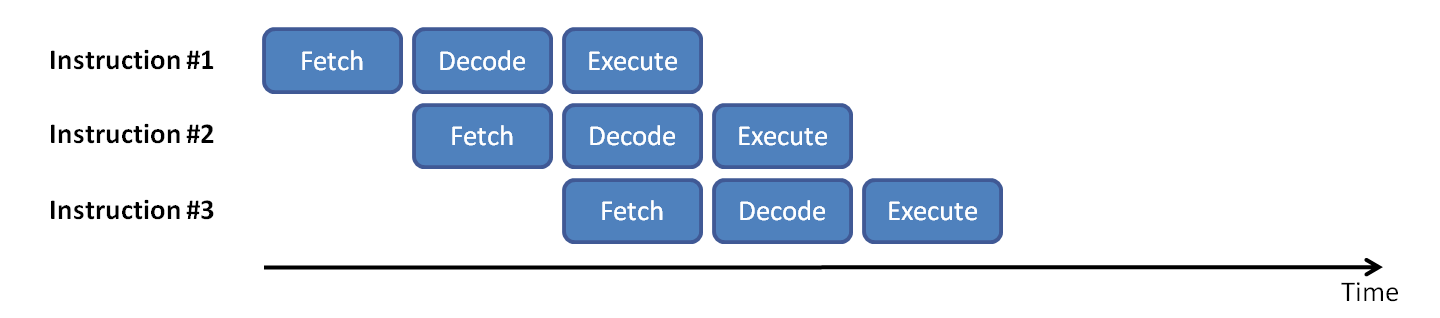
\includegraphics[width=0.6\textwidth]{pipeline}
    \centering
    \caption{Futószalagos végrehajtás}
    \label{fig:pipeline}
\end{figure}
\paragraph{A teljesítmény gátjai:} a gyakorlatban nem mindig valósul meg a fokozatok számának növekedésével arányos gyorsulás.
A végrehajtást a függőségek (adat, vezérlés, erőforrás) lassítják. A függőségek oka a sok párhuzamosan futó utasítás ($n+1$, ahol $n$ a fokozatszám).
\paragraph{A hatékonyság maximalizálása:}a tapasztalat szerint a hatékonyság kb. 15-30 fokozatú futószalag esetén maximalizálható, efölött a függőségek miatt már csökken a teljesítmény.
Ez az általános célú alkalmazásokra igaz, a mai általános processzorokban kb. 20 fokozat van. Speciális feladatokra (ahol kevés a függőség) használható superpipeline CPU, ami akár 200 fokozatú is lehet.

\section{Történeti áttekintés}
\begin{itemize}
    \item Intel 80486: 3 fokozat, de már külön lebegőpontos futószalag
    \item Intel Pentium (P5): 5 fokozat
    \item Intel Pentium III (P6): 11-17 fokozat
    \item Intel Pentium IV (Netburst): 20-31 fokozat
    \item Intel Core 2 (újratervezett P6, több mag): általában 14 fokozat
    \item Intel Core i: 16-20 fokozat
\end{itemize}

\section{Gyakorlati példa - az Intel Atom CPU}
Az Intel Atom processzor a 2000-es években jelent meg, 16 fokozatú futószalagot használ.
A processzor CISC (Complex Instruction Set Computing) architektúrájú, azaz egy utasításon belül nem csak a regiszterekből, hanem a memóriából, vagy a gyorsítótárból is képes adatot lehívni.
\paragraph{Az Intel Atom fokozatai:}
\begin{itemize}
    \item 1-3. fokozat: instruction fetch (IF)
    \item 4-6. fokozat: instruction decode (ID)
    \item 7-8. fokozat: instruction dispatch (SC - Switch Context, IS - Instruction Schedule)
    \item 9. fokozat: source operand read (IRF - Instruction Register File)
    \item 10-12. fokozat: data cache access, CISC architektúrához szükséges (AG - Address Generation, DC\textsubscript{1} - Data Cache 1, DC\textsubscript{2} - Data Cache 2)
    \item 13. fokozat: execute
    \item 14-15. fokozat: exception + multitask handling (FT\textsubscript{1} - Fault Tolerant 1, FT\textsubscript{2} - Fault Tolerant 2)
    \item 16. fokozat: commit, ez a visszaírás (W/B vagy DC\textsubscript{1})
\end{itemize}
\paragraph{Következmény:} ez egy tisztán futószalag elvű processzor, ami teljesítményben visszalépést jelentett a korábbi architektúrákhoz képest.
Előnye az alacsony fogyasztás, ezért főleg mobil eszközökbe használták az Atom CPU-kat.

\section{Futószalagos feldolgozás előfeltételei (2 fokozat esetén)}
Az ideális futószalag megvalósítható, ha
\begin{itemize}
    \item a számítógép 2 db egymástól független végrehajtó egységgel rendelkezik,
    \item az egyik fokozat kimenete a másik fokozat bemenete,
    \item mindkét fokozat végrehajtási ideje azonos,
    \item a fokozatok szinkronizáltak, órajelre kapják az inputot, és egyetlen óraciklus alatt elvégzik a feladatukat.
\end{itemize}
Ekkor $t=\frac{T}{2}$, ahol $T$ a szekvenciális végrehajtási idő és $t$ a futószalagos végrehajtási idő.

\section{Függőségek kezelése}
\begin{itemize}
    \item Operandus előrehozással:
    \begin{itemize}
        \item Minden architektúránál használják.
        \item Részletesen: \ref{fuggosegek}. fejezet.
    \end{itemize}
    \item Újrafeldolgozással:
    \begin{itemize}
        \item Leggyakrabban az execute fokozat egymás után többszöri végrehajtását jelenti.
        \item Pl. szorzásnál az ismétlődő összeadásokhoz használható.
        \item A futószalag feldolgozást lassítja, de összességében jobb teljesítményt biztosít.
    \end{itemize}
\end{itemize}

\section{Típusai}
\begin{enumerate}
    \item Előlehívás (overlapping)
    \item Vektor CPU-k (60-as évek)
    \item Teljes pipeline
\end{enumerate}

\subsection{Előlehívás}
A visszaírás során történik meg a következő utasítás lehívása:
\begin{center}
    \begin{tabular}{ c | c | c | c | c | c | c | c }
        & t\textsubscript{1} & t\textsubscript{2} & t\textsubscript{3} &t\textsubscript{4} & t\textsubscript{5} & t\textsubscript{6} & t\textsubscript{7} \\
        \hline
        I\textsubscript{1} & F & D & E & W/B \\
        \hline
        I\textsubscript{2} &   &   &   & F & D & E & W/B
    \end{tabular}
\end{center}
\paragraph{Előnyök:}
\begin{itemize}
    \item 4 óraciklus helyett csak 3 kell egy utasításhoz, így a teljesítmény 25\%-al nő, valamint
    \item nincsenek függőségek, mivel a forrás operandus beolvasásakor (t\textsubscript{5}) már megvan az előző utasítás eredménye (t\textsubscript{4}).
\end{itemize}
\paragraph{Hátrány:} nem túl nagy mértékű gyorsulás.

\subsection{Vektor CPU}
Csak az execute fokozat működött futószalagszerűen.

\subsection{Teljes pipeline}
A futószalagos feldolgozás kiterjesztése a teljes folyamatra:
\begin{center}
    \begin{tabular}{ c | c | c | c | c | c  }
        & t\textsubscript{1} & t\textsubscript{2} & t\textsubscript{3} &t\textsubscript{4} & t\textsubscript{5} \\
        \hline
        I\textsubscript{1} & F & D & E & W/B \\
        \hline
        I\textsubscript{2} &   &  F & D & E & W/B
    \end{tabular}
\end{center}

\section{Logikai futószalagok} \label{logikai_futoszalag}
Az eltérő utasítások eltérő felépítésű futószalagokat igényelnek, ezért egy processzor több futószalagot is tartalmaz.
A cél a funkcionális kialakítás. Példák különböző funkciókat ellátó futószalagokra:
\begin{itemize}
    \item aritmetikai: F, D, E, W/B
    \begin{itemize}
        \item fixpontos
        \begin{itemize}
            \item egyszerű: +, -, léptetés, ...
            \item összetett: *, /, ...
        \end{itemize}
        \item lebegőpontos
    \end{itemize}
    \item ugró (branch): F, E
    \item LOAD / STORE
\end{itemize}
\paragraph{Az utasítások értelmezése:} az utasításokat két szinten értelmezhetjük, pl. a fetch utasítás két szintje a következő:
\begin{enumerate}
    \item Fetch
    \item MAR $\leftarrow$ PC\\
    MDR $\leftarrow$ [MAR] \\
    IR $\leftarrow$ MDR \\
    PC $\leftarrow$ PC+1
\end{enumerate}

\section{Fizikai megvalósítás}
Alkalmazásuk alapján megkülönböztetünk univerzális és dedikált futószalagokat.
Az univerzális minden művelet elvégzésére alkalmas, míg a dedikált speciális műveletekre képes.
Hardveres szempontból az univerzális futószalag előnytelen, mivel sok tranzisztorra van szükség, a kialakítása bonyolult és drága, ráadásul a végrehajtás lassú.
Ezért általában a \ref{logikai_futoszalag}. részben leírt dedikált (egy adott funciót ellátó) futószalagokat építenek a processzorokba.
Az eredmény kevesebb logikai kapu, így gyorsul a végrehajtás (a bemenettől a kimenetig gyorsabban átérnek az elektronok).
\paragraph{Megjegyzés:} a futószalag sebességét általában a leglassabb fokozat sebessége határozza meg, tehát a tervezési cél a megközelítőleg azonos sebességű fokozatok létrehozása.
\paragraph{Fokozatok kialakítása:} a fokozatok előtt előválasztó (puffer) regiszterek vannak. Ezek a felhasználó számára láthatatlanok, az adat először ezekbe töltődik be.
Ezekből a regiszterekből kerül aztán a végrehajtó egységbe az adat, majd az utasítás elvégzése után szintén puffer regiszterekbe kerül a kimenet.
A puffer regiszterek szükségesek, mivel a gyakorlatban egy fokozat nem mindig végez egy óraciklus alatt.
Az ebből adódó várakozás során ezekben a regiszterekben tárolódik az adat.
Ennek a kialakítása látható a \ref{fig:fokozat}. ábrán. A későbbiekben a végrehajtó egységekből egymás mellé többet is helyeztek, így megvalósítva a térbeli párhuzamosságot (\ref{fig:fokozat_parhuzamos}. ábra).
\begin{figure}[h]
    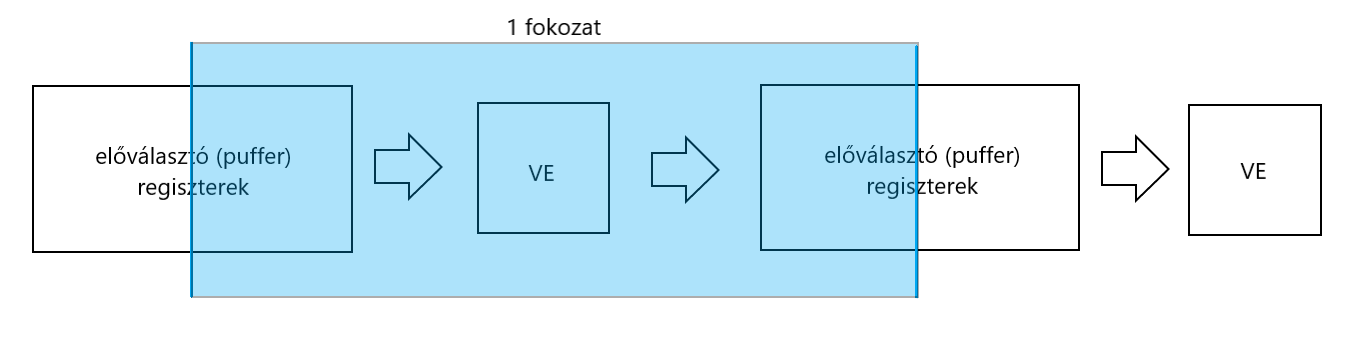
\includegraphics[width=0.6\textwidth]{fokozat}
    \centering
    \caption{A fokozatok felépítése}
    \label{fig:fokozat}
\end{figure}
\begin{figure}[h]
    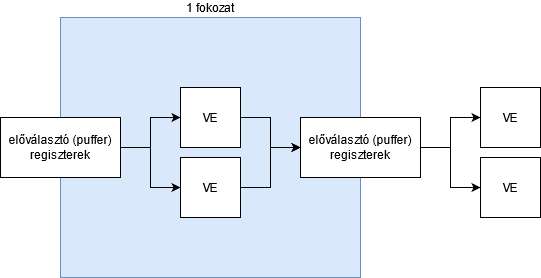
\includegraphics[width=0.6\textwidth]{fokozat_parhuzamos}
    \centering
    \caption{A végrehajtó egységek párhuzamosítása}
    \label{fig:fokozat_parhuzamos}
\end{figure}

\subsection{Példa: a PowerPC 604}
A PowerPC 604-es processzorban egymással párhuzamosan több dedikált futószalag is működött (\ref{fig:powerpc604} ábra).
A fetch és decode fokozatok minden óraciklusra lehívtak egy utasítást, és a megfelelő futószalagba töltötték.
Így a CPU képes volt egymással párhuzamosan több utasítást is végrehajtani (akár 4-et is).
Mivel előfordulhatott, hogy a később lehívott és betöltött utasítás végzett hamarabb (pl. elsőként egy FP, másodikként egy FX utasítás $\rightarrow$ FX hamarabb végez), szükséges volt egy konzisztencia fokozat (CO) bevezetése.
Az utasítások címkézésre kerültek, a sorrendet a CO biztosította.
A párhuzamosság miatt szükség volt a fokozatok közötti várakoztatásra, ez az interlock funkció.
\paragraph{Megjegyzés:} az Intel 80486 és az első Pentium csak 2 utasítás futószalaggal rendelkezett. A mai Core i architectúrák magonkánt általában 6-8 futószalagot alkalmaznak.
\label{powerpc604}
\begin{figure}[H]
    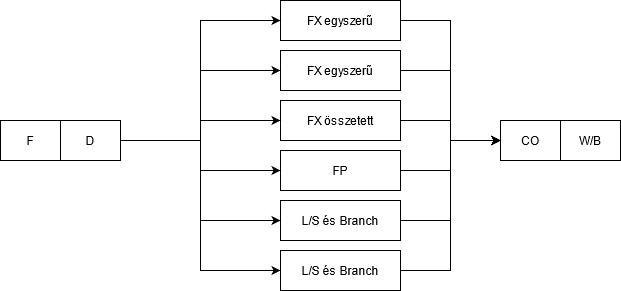
\includegraphics[width=0.6\textwidth]{powerpc604}
    \centering
    \caption{A PowerPC 604 futószalagja}
    \label{fig:powerpc604}
\end{figure}

\section{RISC és CISC architektúrák}
Az utasításkészlet (tervezési stratégia) alapján kétféle architektúrát különböztetünk meg:
\begin{itemize}
    \item RISC: Reduced Instruction Set Computing - csökkentett utasításkészletű architektúra és
    \item CISC: Complex Instruction Set Computing - bővített utasításkészletű architektúra.
\end{itemize}
Mindkettő használatban van napjainkban.
\subsection{Történeti áttekintés}
Az első CPU-k kevés utasítással rendelkeztek (RISC), majd a 70-es években az egyre több funkció és bonyolultabb utasítások miatt ez a szám növekedett (CISC).
A 80-as években rájöttek, hogy a sok utasítás ugyan megkönnyíti a programozást, de a címzés bonyolultsága miatt káros hatással van a teljesítményre.
Ez vezetett a RISC architektúrák újbóli megjelenéséhez.

\subsection{RISC}
\paragraph{Példa:} a mobil eszközök ARM (Advanced RISC Machine) processzorai RISC architektúrájúak.
\paragraph{Tulajdonságai:}
\begin{itemize}
    \item Kis számú (50-150) utasítással rendelkezik $\rightarrow$ címzési módok egyszerűsödése.
    \item Nincs olyan utasítás, ami a LOAD/STORE-t aritmetikával kombinálja (nem lehet egyszerre betölteni az adatot és végrehajtani a műveletet).
    \item Minden műveletvégző utasítás regisztereket használ $\rightarrow$ memóriából vagy gyorsítótárból nem lehet dolgozni.
    \item Memória vagy cache elérés csak LOAD/STORE utasításokkal történhet.
    \item Nagy számú regiszterkészlet (mivel minden művelethez regiszterekre van szükség).
    \item Általában 3 operandusos utasítások $\rightarrow$ az eredmény nem írja felül a bemeneti regisztert, hanem külön regiszterbe kerül.
    \item Minden utasítás hossza egyforma (pl. 128 bit) $\rightarrow$ könnyebb a futószalagos feldolgozás.
    \item A fordítóprogramok bonyolultabbak a kevés utasítás miatt.
    \item Általában huzalozott (hardveres) az utasítás feldolgozás (decode).
    \item Utasítás végrehajtás általában egy óraciklust vesz igénybe (cél az egyforma ciklusidő).
\end{itemize}
\paragraph{Előnye:} általában gyorsabb végrehajtás a CISC architektúrákhoz képest.
\paragraph{Hátránya:} a bonyolultabb feladatokat instrukció szekvenciákkal kell megoldani.
Ez a fordításnál okoz problémát, növelheti a program méretét.

\subsection{CISC}
\paragraph{Példa:} a 80-as években elterjedt Intel 80386-os egy tisztán CISC architektúra.
\paragraph{Tulajdonságai:}
\begin{itemize}
    \item Nagy számú utasításkészlet (több száz).
    \item A sok utasítás nagy belső mikroprogramtárat igényel.
    \item Sokféle címzési mód (tartalmaz típus címzési módot is) és sokféle utasítás.
    \item Változó méretű (akár összetett) utasítások $\rightarrow$ a dekódolónak nem csak dekódolni kell az utasítást, hanem azonosítani is az utasítás végét (tudnia kell, hogy hol fejeződik be). Ezt hívják utasítás határra illesztésnek, plusz hardvert és időt igényel.
    \item Közvetlen memória elérés lehetsége $\rightarrow$ a második operandus lehet memória vagy cache cím is.
    \item Két operandusos utasítások $\rightarrow$ az első operandus felülíródik az eredménnyel.
    \item Az előző kettőből következik, hogy az első operandus nem lehet memória/cache cím, mivel az eredmény memóriába írása nagyon lelassítaná a működést.
    \item Az utasítások feldolgozása több ciklusidő lehet $\rightarrow$ bonyolultabb feldolgozás.
    \item Egyszerűbb a gépi kódú programozás a sokféle utasítás miatt (egyszerűbb fordítóprogramok).
    \item Egy utasításban több elemi műveletet is végre tud hajtani.
    \item Az utasítások folyamatosan bővültek, így a régi programokkal visszafelé kompatibilis maradt.
    \item A futószalag fokozatok között sebesség különbség lehet $\rightarrow$ feloldására interlock funkciót használnak (részletesen: \ref{powerpc604}).
    \item Általában a memória elérés miatt +2 fokozat szükséges a RISC-hez képest (AG - címszámítás és cache elérés).
\end{itemize}
\paragraph{Előnyei:} kompatibilitás a régi programokkal, egyszerűbb compilerek.
\paragraph{Hátránya:} bonyolultabb, lassabb végrehajtás.

\subsection{Hibrid CISC}
\paragraph{Példa:} az x86-os architektúra ISA-t (Instruction Set Architecture) használ, ami egy hibrid CISC architektúra.
\paragraph{Tapasztalat:} megfigyelték, hogy a CISC processzorok az idő 80\%-ában az utasítások mindössze kb. 20\%-át használják.
\paragraph{Optimalizálás:} a feldolgozás gyorsítása érdekében kialakítottak a CISC architektúrán belül egy RISC magot.
Ez a megoldás minden mai (Core i) architektúrában megjelenik.

\subsection{Hibrid RISC}
A mai ARM processzorok sem tisztán RISC architektúrák, hanem CISC jellegű utasításokkal vannak kibővítve (pl. az ARM Thumb, ami egy tömörített utasításkészlet).

\section{Következmények}
A futószalagos feldolgozás következményei:
\begin{itemize}
    \item Jelentősen felgyorsult az utasítások lehívása és az operandusok betöltése.
    \item Amíg a processzorok feldolgozási sebessége jelentősen nőtt, a memória sebessége kevésbé (ez a jelenség a sebességolló) $\rightarrow$ cache bevezetése (IBM - 1968, Intel - 80-as évek). A cache előnye, hogy a gyakran használt operandusok gyorsan elérhetők.
    \item Maximális végrehajtási sebesség: 1 utasítás / ciklus (további növekedés kibocsátási párhuzamossággal vagy utasításon belüli párhuzamossággal lehetséges).
    \item A vezérlés átadási utasítások kifinomult technikája szükséges (függőségek miatt).
    \item Az elágazás kezelés bonyolódik.
\end{itemize}

\subsection{Elágazások kezelése}
\subsubsection{Korai RISC gépek}
Kezelés ugrási buborékkal.
\subsubsection{Korai CISC gépek}
A dekódoló fokozatba építették a címszámító és a logikai komparáló egységet, így a dekódolási ciklus végére előáll az ugrási cím.
\subsubsection{Későbbi CISC gépek (futószalag CPU-k és első generációs szuperskalár architektúrák)}
Kezelés fix előrejelzéssel, pl. mindig ugrik.
Ezzel a megoldással az ugrási cím előre kiszámításra kerül és megkezdődik az ugrási címen lévő utasítások lehívása.
Ha mégse kell ugrani, az utasításokat visszatörli és az eredeti helyen folytatódik a végrehajtás.
Előnye, hogy kiküszübölte az ugrási buborékot, növekszik a teljesítmény.
Korlátja, hogy ha nagy látenciával rendelkező műveletet kellett végrehajtani az ugrási feltételben, az blokkolta a kibocsátást.
Ilyen megoldást használ például az Intel 80486-os CPU.
\subsubsection{Második generációs szuperskalár architektúrák}
A CPU a dekódolási folyamatok egy részét már akkor elvégzi, amikor az utasításokat az L1 cache-be írja.
Az előre elvégzett feladatok:
\begin{itemize}
    \item utasítás típusazonosítás
    \item ugrások felismerése
    \item utasításhossz meghatározása (szükséges, mivel CISC-nél változó az utasításhossz)
    \item spekulatív elágazásbecslés
    \begin{itemize}
        \item regiszterátnevezéssel
        \item átrendező puffer (Intel: ROB - ReOrder Buffer)
    \end{itemize}
\end{itemize}

\section{Összegzés}
A fejezetben felsorolt módszerekkel elérték a futószalag elvű processzorok teljesítményének korlátait.
A további gyorsítás érdekében párhuzamos kibocsátást kellett alkalmazni, így jöttek létre a szuperskalár processzorok.